\chapter{Tecnologias Utilizadas}
\section{Desenvolvimento}
	\subsection{NodeJS}
	\subsection{AngularJS}
	\subsection{Material Design}
	\subsection{Plugins JS}
		\paragraph{Johnny5} 
		\paragraph{Genisys}
		\paragraph{AngularFire}
		\paragraph{AngularMaterial}
	\section{Cloudmqtt}
		\subsection{MQTT}
	\section{Firebase}
		\subsection{Database/ Pub-Sub}
	\section{Prot\'otipos}
		\subsection{Arduino}
		\subsection{NodeMCU}
		\subsection{Firmata firmware}
	\section{Sensors}
	\subsection{sub-item x}
	\section{Processamento dos dados}
		\subsection{Apache Kafka}
		Ferramenta projetada para funcionar como um midleware de mensageria (Figura~\ref{fig:arqkafka}), utilizando o padr\~ao Publish/Subscribe para criar canais ("streams") de mensagens entre v\'arias origens diferentes ("Producers") e os v\'arios destinos inscritos ("Consumers").
		
		\begin{figure}[ht]
			\centering
			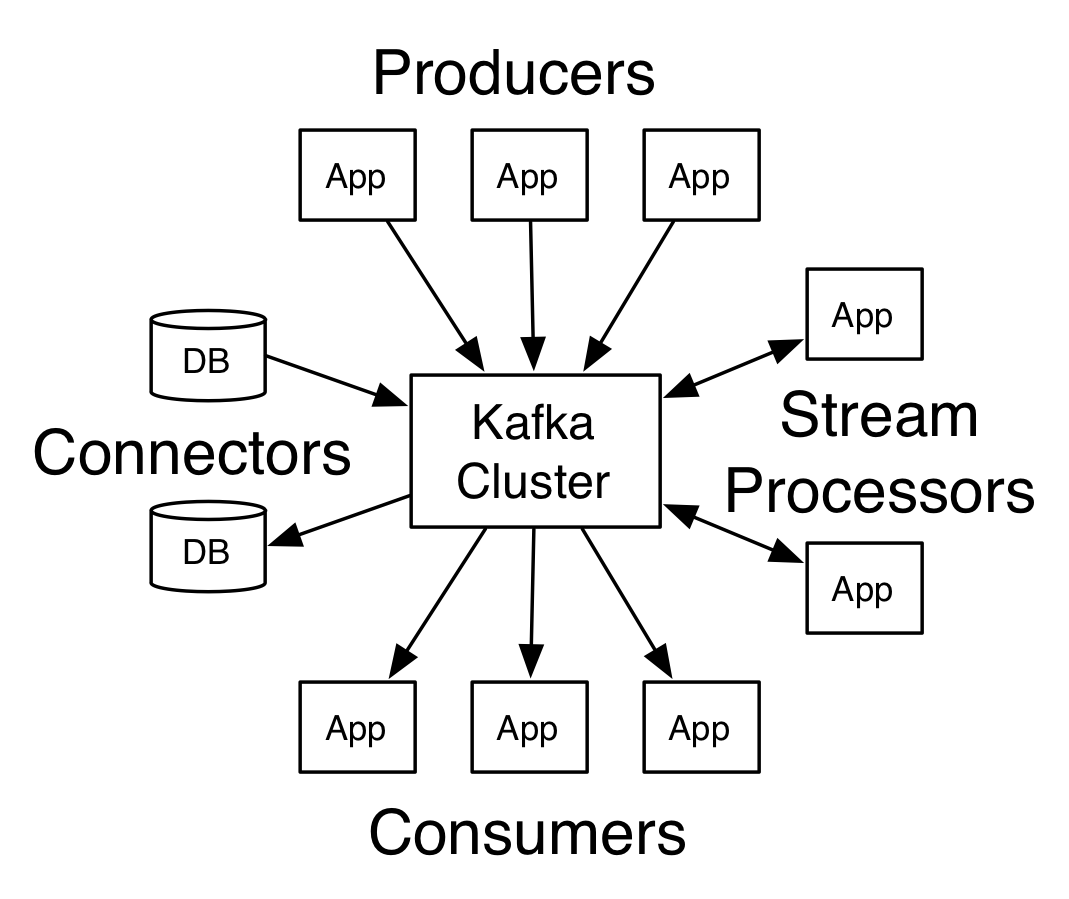
\includegraphics[width=.5\textwidth]{fig0.png}
			\caption{Arquitetura do Kafka}
			\label{fig:arqkafka}
		\end{figure}
		
		Com a utiliza\c{c}\~ao de conectores, bancos de dados podem ser utilizados para persist\^encia de mensagens e ao conect\'a-lo à ferramentas de \'analise e processamento de dados ("Stream Processors"), suas mensagens podem ser transformadas antes de sua publiblica\c{c}\~ao.
		
		Dentre os principais benef\'icios da ferramenta est\~ao: publica\c{c}\~ao em tempo real, funcionamento distribu\'ido em um ou mais servidores, separa\c{c}\~ao dos canais em categorias/t\'opicos, possui recursos de particionamento tolerantes à falhas e garantia na entrega das mensagens com replica\c{c}\~ao de dados. 
		
		\subsection{Apache Storm}
		Essa ferramenta Open Source pode ser utilizada na execu\c{c}\~ao de tarefas em paralelo de forma continua, que \'e o caso de grande parte dos projetos de IoT. Seus Fluxos de trabalhos ou "Topologias", devem ser projetados a partir de grafos ac\'iclicos direcionados (DAG's) que ao entrar em execu\c{c}\~ao, realizam suas tarefas indefinidamente processando os dados gerados pelos dispositivos ub\'iquos de forma cont\'inua. Suas topologias s\'o param de rodar em 2 casos, a partir da interven\c{c}\~ao do usu\'ario matando seu processo ou na ocorr\^encia de uma falha irrecuper\'avel. 
		
		Sua topologia \'e formada por "spouts" ou "bolts" como seus v\'ertices, enquanto que suas arestas representam fluxos de dados trafegados entre os n\'os do grafo. Em conjunto, v\'ertices e arestas da topologia agem como um pipeline de transforma\c{c}\~ao dos dados em tempo real(Figura~\ref{fig:arqstorm}).
		
		\begin{figure}[ht]
			\centering
			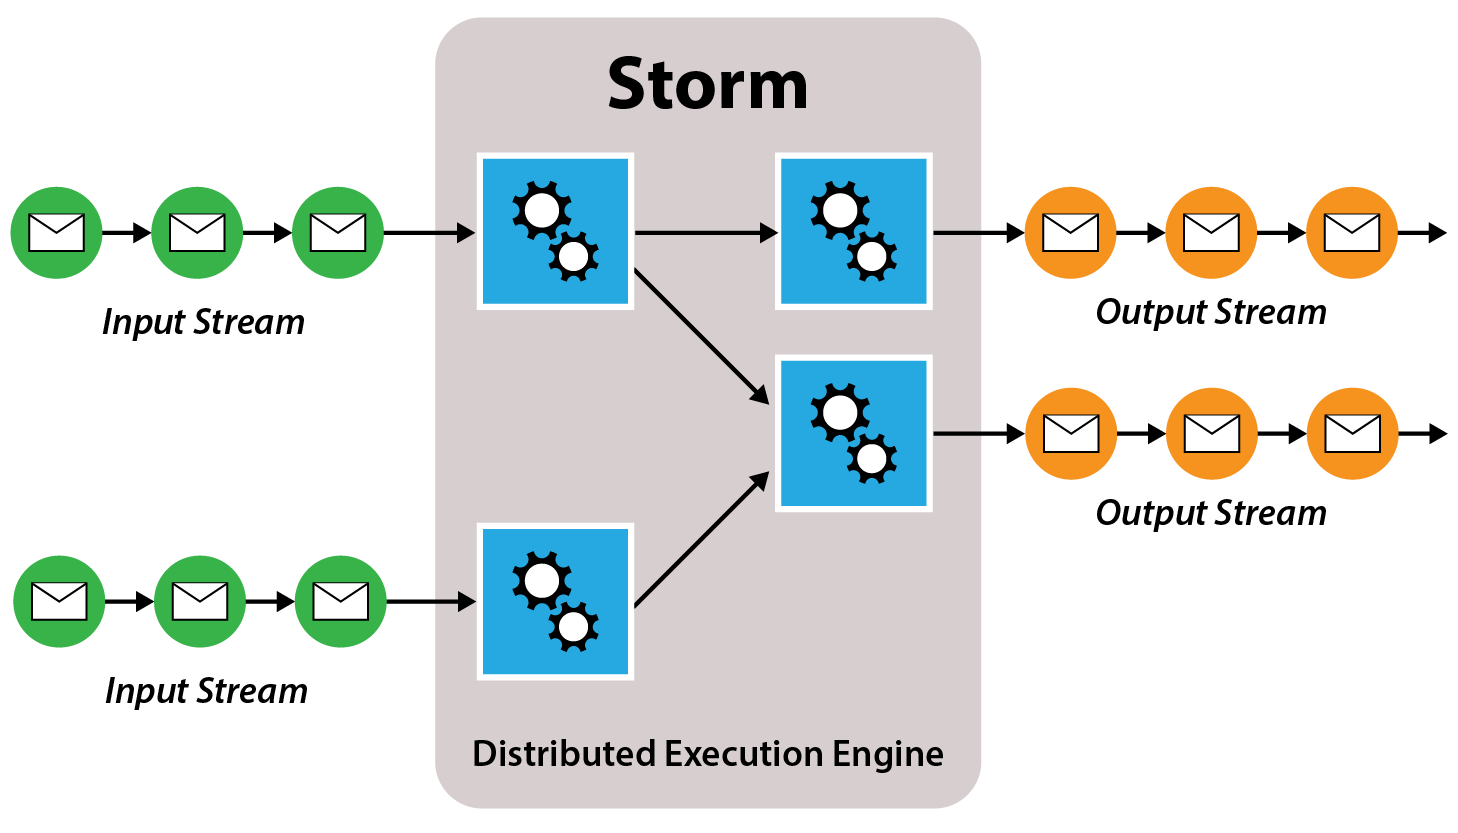
\includegraphics[width=.5\textwidth]{fig4.png}
			\caption{Exemplo de topologia no Storm}
			\label{fig:arqstorm}
		\end{figure}
		
		O Storm n\~ao possui suporte nativo aos clusters do Hadoop/YARN (Ainda em desenvolvimento), ao inv\'es disso ele usa a estrutura da ferramenta Zookeeper e seus pr\'oprios processos de trabalho (master/minion) para coordena\c{c}\~ao de suas topologias, estados e mensagens sem\^anticas de garantia. Al\'em disso, ele pode consumir e escrever arquivos no HDFS e tamb\'em rodar nativamente sobre o gerenciador de cluster Apache Mesos ou com o suporte da plataforma de orequestra\c{c}\~ao de containers Marathon.